\section{Tutorial}
\label{tutorial_csp}

The objective of this chapter is to get you to a stage where you can use BMotion Studio to visualize CSP-M models. 
We expect that you have already downloaded the BMotion Studio tool (see Section~\ref{installation}) and created a new visualisation template for Event-B visualisations (see Section~\ref{vis_template}).
 
%We expect you to have a basic understanding of logic and an idea why doing formal modelling is a good idea.  
You should be able to work through the tutorial with no or little outside help.

We encourage you not to download solutions to the examples but instead to actively build them up yourself as the tutorial progresses.

If something is unclear, remember to check the Reference (\ref{reference_csp}) for more information.

\subsection{Preparation}

Let's start by creating a new visualisation template as described in Section~\ref{vis_template}.
Just duplicate the \texttt{csp\_template} folder and rename it to \texttt{bully}.
After refreshing your browser, a new folder called \texttt{bully} should appear in your workspace.

\subsection{The Formal Model}

We are going to create a visualisation of the bully algorithm specification found in the book ``Understanding Concurrent Systems'' (ISBN 978-1-84882-258-0).
The algorithm represents a method of distributed computing for electing a node to be the coordinator amongst a group of nodes.
Each node has a unique ID and the algorithm intends to select the node with the highest ID to be the coordinator.
It is assumed that the nodes may fail and revive from time to time and the communication between the nodes is reliable.
Three types of messages are defined within the design of the algorithm: \textit{election} (announcing an election), \textit{answer} (responding to an election message), and \textit{coordinator} (announcing the identity of the coordinator).

The bully algorithm specification defines six additional types of events needed for the formalisation of the algorithm in CSP:
the \textit{fail} and \textit{revive} events (for modelling failing and reviving of a node), the \textit{test} and \textit{ok} events (for simulating a test-response communication), the \textit{leader} events (for indicating the coordinator of a living node), and the \textit{tock} event (for modelling timeouts and time).

You can download the CSP model \file{BullyAlgorithm.zip}{here}.
Decompress it and put the files into a new folder called \texttt{model} relative to your \texttt{template.html} file in your workspace.

\subsection{Linking the Model with the Visualisation}

The next step consists of linking the model with the visualisation.
For this, open the \texttt{template.html} file with an HTML/text editor of your choice and add the following line within the head tag:

\begin{lstlisting}[language=html]
<meta name="bms.model" content="model/bully.csp" />
\end{lstlisting}

We link the visualisation with the CSP-M model called ``bully.csp''.

\subsection{Creating the Actual Visualisation}
\label{tutorial_csp_create_vis}

The next step consists of creating the actual visualisation.
The user is not restricted to an editor in order to create a visualisation.
The user can make use of any tool that support the creation of SVG graphics or HTML documents.
Please download the prepared \file{bully.svg}{bully.svg} file.
Feel free to modify and explore the SVG graphic.
Open the SVG file with a text editor of your choice and put the SVG code within the body tag in the \texttt{template.html} file located in your workspace.

\begin{figure}[h!]\centering
	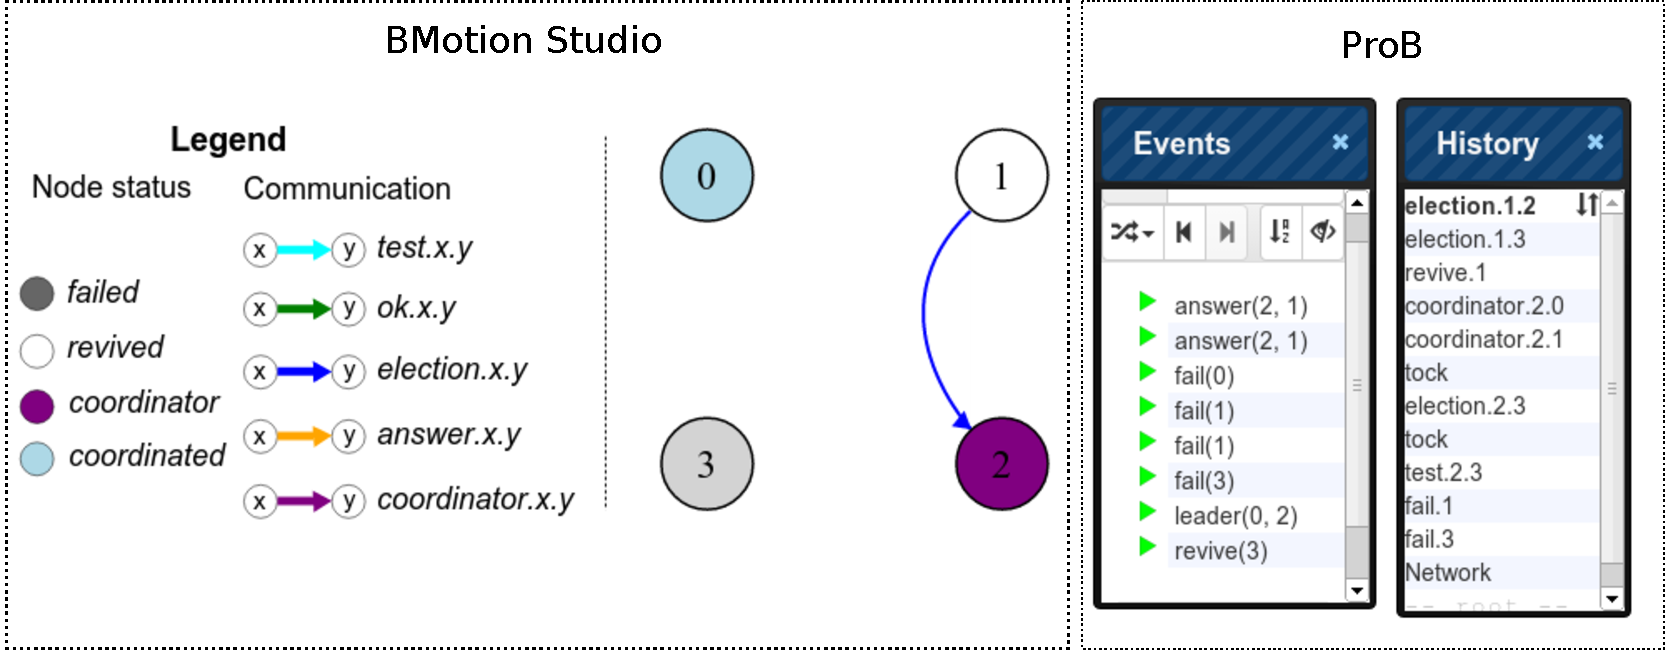
\includegraphics[width=\textwidth]{img/tutorial/runningvis}
	\caption{The final Bully Algorithm Visualisation}
	\label{fig:BullyVisState}
\end{figure}

In general, we want to visualise the process of electing a leader in the network.
More precisely, we aim to visualise the $Network$ process of the CSP specification.
As the bully algorithm specification is presented for a network with four nodes, we also intend to create a visualisation for four nodes (the nodes are enumerated from 0 to 3). 
Fig.~\ref{fig:BullyVisState} demonstrates the visualisation of a particular trace.

There are two major aspects of the specification that we want to visualise: the nodes and the communication between the nodes.
Each node is visualised by means of a circle in which the respective ID is positioned, whereas the communication between the nodes is illustrated by directed arrows.
Each directed arrow is made up of a line and a corresponding arrowhead.

To each visual element in the visualisation we assign a unique ID referring to the elements in the CSP specification.
Thus, the node with ID $x$ in the CSP specification is presented by the circle with ID "n-x" in the visualisation.
Additionally, a message transfer from the node with ID $x$ to the node with ID $y$ is represented by the line with ID "l-x-y" and the arrowhead with ID "p-y" (i.e. the arrow connecting "n-x" and "n-y").
In this section, both symbols $x$ and $y$ stand for an integer ranging from 0 to 3.

We can classify all types of events in the specification into the following groups:
\begin{itemize}
\item \textbf{status:} Events that can change the status of a particular node $x$: $fail.x$, $revive.x$, $coordinator.x.y$, and $leader.x.y$.
\item \textbf{message:} Events illustrating a message transfer from node $x$ to node $y$: $test.x.y$, $ok.x.y$, $election.x.y$, $answer.x.y$, and $coordinator.x.y$.
\item \textbf{hidden:} Events that are not considered in the visualisation: $tock$.
\end{itemize}
Thus, we can infer that there are two general types of observers to define: the \textit{status} and the \textit{message} observers.
Note that each \textit{coordinator} event (\textit{coordinator.x.y}) has been included in the first two groups above. 
This is because in the specification each of the \textit{coordinator} events intends to identify the coordinator ($x$) and at the same time represents a message transfer (to node $y$).

The status of a node usually changes when one of the \textit{status} events has been executed.
Each node, except for the node with the lowest ID\footnote{The node with ID 0 can never be a coordinator as there is no node with a lower ID.}, can have the following status: \texttt{failed}, \texttt{revived}, \texttt{coordinator}, or \texttt{coordinated}.
A unique colour has been selected for distinguishing each possible status of a node (see legend in Fig.~\ref{fig:BullyVisState}).
For instance, the node with ID ``n-3'' will be coloured in grey when the event $fail.3$ has been processed.

\subsection{Creating Observers}

Start with adding a new CSP event observer on the visual element that matches the selector ``\#bully''.
Add the following JavaScript code to your \texttt{template.js} file:

\begin{lstlisting}[language=JavaScript]
$("#bully").observe("csp-event", {
  observers: []
});
\end{lstlisting}

The visual element that matches the selector ``\#bully'' defines the parent for the CSP event observer.
In particular, the selector matches the SVG element (the actual visualisation) that we added in the previous Section~\ref{tutorial_csp_create_vis}.

In order to associate a \textit{status} event from the CSP specification with a node in the visualisation, we use the selector ``\#n-\{\{a1\}\}'' in the definition of the respective observer. The construct ``\{\{a1\}\}'' is used in the selector for obtaining the value of the first argument of the respective \textit{status} event.
For example, the observer for changing a status of a node to \texttt{failed} can be defined as follows:

\begin{lstlisting}[language=JavaScript]
{
  exp: "{fail.x | x <- {0..N-1}}",
  actions: [
    { selector: "#n-{{a1}}",
      attr: "fill",
      value: "lightgray"
    }
  ]
}
\end{lstlisting}

Add this observer in the list of observers.

In a similar fashion we have defined the observers for the other node status changes. 

For creating the \textit{message} observers we need to consider both arguments of the \textit{message} events.
The types of the messages are distinguished by different stroke patterns (see Fig. \ref{fig:BullyVisState}).
Thus, each \textit{message} observer, except for the \textit{coordinator} observer (this observer has three actions), has two actions: one action for appearing the arrow (the line and arrowhead constituting the respective arrow in the visualisation) and one action for changing the color of the arrow.
For instance, the observer for visualising the election message can be defined as follows:

\begin{lstlisting}[language=JavaScript]
{
  exp: "{election.x.y | x <- {0..N-1}, y <- {0..N-1}}",
  actions: [
    { selector: "#l-{{a1}}-{{a2}}, #p-{{a2}}",
      attr: "class",
      value: "visible"
    },
    { selector: "#l-{{a1}}-{{a2}}",
      attr: "stroke",
      value: "blue"
    }
  ]
}
\end{lstlisting}

To provide a clear visualisation an additional observer has been added to hide all arrows after performing an arbitrary event.
This observer is applied on the currently processed event before all other defined observers:

\begin{lstlisting}[language=JavaScript]
{
  exp: "Events",
  actions: [
    { selector: "path[id^=l-], path[id^=p-]", 
      attr: "class", 
      value: "hidden"
    }
  ]
}
\end{lstlisting}
 
The initial state of the specification and the visualisation is the state in the network where all nodes are alive and the coordinator is the node with the ID 3 (the node with the greatest ID). 
Additionally, no message exchanges are performed.